\documentclass[output=paper]{langscibook}
\ChapterDOI{10.5281/zenodo.6762276}

\author{Todd A. Hernández\affiliation{Marquette University}}
\title{Measuring L2 pragmatic development in the study abroad context}
\abstract{Although it is often assumed that study abroad (SA) provides an ideal environment for second language (L2) pragmatic development, research has demonstrated that students’ lack of consistent exposure to the target language imposes limitations on such development (\citealt{Barron2003,KasperRose2002,Shively2010}). Further, studies have found that even highly motivated SA are often unaware of how to take full advantage of the SA environment to strategically develop their pragmatic competence (\citealt{CohenShively2007,Hernández2016,Shively2010}). Given this background information, it is clear that programs must develop reliable models for assessing the effects of the SA experience on pragmatic development and other L2 outcomes as well.

I begin this chapter with an overview of pragmatic competence in the SA context. This chapter then focuses on methods of assessing L2 pragmatic development in SA environments. I review and provide examples of research that employs a wide range of assessment methods, from discourse completion tasks (DCTs) and controlled production tasks to role-plays and more open-ended production tasks and naturalistic data. In addition, retrospective verbal reports, language contact profiles, and journal entries are discussed as tools that can inform and improve SA participants’ learning. I then discuss studies that have assessed the impact of pedagogical intervention on SA students’ L2 pragmatic development. I conclude this chapter with a discussion of the implications of SA assessment of pragmatic development and outline directions for future research.
\keywords{pragmatic development, study abroad, assessment, language learning}
}

\begin{document}
\AffiliationsWithoutIndexing{}
\maketitle




\section{Introduction}

Pragmatic competence, a core feature of communicative competence and a central goal of foreign language instruction (\citealt{BachmanPalmer1996}, Canale \& Swain \citeyear{CanaleSwain1980}), refers to “one’s knowledge of linguistics, norms, and social conventions, and one’s ability to use these knowledge bases in a socially-bound interaction” \citep[1]{Taguchi2015}. Second language (L2) learners interested in achieving native-like competence in a target language must acquire two distinct yet related knowledge bases: pragmalinguistic knowledge, or knowledge of the specific forms and linguistic strategies involved in the performance of a speech act (e.g., how to refuse an invitation), and sociopragmatic knowledge, or knowledge of the social norms of a culture and how they influence interactional patterns \citep{Thomas1983}.

Study abroad (SA), a formal educational experience by a student in a target language country, is often considered an ideal context for L2 pragmatic development because it has the potential to provide SA learners with access to large amounts of input and interaction with native speakers (\citealt{Hernández2010,Ren2018,VandeBergLou2012}). SA is “characterized by an uninstructed (i.e., implicit) component that may or may not combine with an instructed (i.e., explicit) component” (\citealt[1]{Sanz2014}). More than in the foreign language classroom, L2 learners have frequent opportunities during SA to use the target language to perform a wide range of speech acts or communicative functions (e.g., apologies, compliments, requests, refusals) that have real-world consequences \citep{Shively2011}. Although previous research has shown that SA has a positive impact on L2 pragmatic development for some learners, there is considerable individual variation in outcomes (e.g., \citealt{Barron2006,Bataller2010,Félix-BrasdeferHasler-Barker2015,Hernández2018b,ShivelyCohen2008}). SA assessment research has identified several factors that contribute to this variation: “quantity and quality of contact with the L2, length of stay, living situation, density of L2 speaking social networks, and individual characteristics (e.g., proficiency, motivation, gender, age, identity, dispositions)” (\citealt[355]{PérezVidalShively2019}). Learner agency has also been proposed as having an influence on L2 pragmatic development (\citealt{LoCastro2003,LoCastro2012}). That is, SA learners may choose not to adopt target pragmatic norms when the norms contradict their social identity (e.g., \citealt{Bataller2010}). Finally, the fact that SA students often do not receive corrective feedback from native speakers about pragmatics and are thus frequently unaware that their language use does not conform to host culture norms represents yet another challenge to L2 pragmatic development in the SA context (\citealt{HernándezBoero2018b,Shively2010}).

This chapter offers an overview of studies that have measured L2 pragmatic development in the SA context. The first section discusses several assessment methods that have been employed to measure SA participants’ pragmatic competence. A review of the existing literature on uninstructed and instructed L2 pragmatic development follows. Some suggested avenues of future research are then given.

\section{Data collection methods for assessing L2 pragmatic competence in SA}

 Given the social nature of pragmatic competence, one of the challenges re\-search\-ers face in measuring pragmatic knowledge concerns collecting data “that closely reflects L2 learners’ language use in social contexts” (\citealt[7]{Taguchi2018}). While experimental data are often criticized for their lack of authenticity, a disadvantage of naturalistic data is their lack of generalizability or comparability (\citealt{Taguchi2018,TaguchiRoever2017}). Data collection methods commonly used to assess SA participants’ L2 pragmatic competence include: written discourse completion tasks (DCTs) (e.g., \citealt{CohenShively2007,Hernández2016,Hernández2018a,HernándezBoero2018a,ShivelyCohen2008}); oral DCTs (ODCTs; e.g., \citealt{Félix-BrasdeferHasler-Barker2015,Halenko2018,Hernándezinpress,TaguchiLi2016}) and multimedia elicitation tasks (METs; e.g., \citealt{Schauer2004}); role-plays (e.g., \citealt{Bataller2010,Hernández2018b,Woodfield2012}); audio recordings of tasks performed abroad (e.g., \citealt{HernándezBoero2018a,Morris2017}); journal entries (e.g., \citealt{Dufon1999,Hernández2018b,Shively2011}); naturalistic data (e.g., \citealt{Dufon1999,Shively2011,Shively2015,Shively2015});  retrospective verbal reports (RVRs; e.g., \citealt{Hernández2018a,Ren2014,Woodfield2012}); and native speaker perceptions of pragmatic appropriateness (e.g., \citealt{CohenShively2007,Hernández2016,Hernández2018a,Hernándezinpress,HernándezBoero2018a,Li2014,ShivelyCohen2008,Taguchi2011}).

 DCTs, sometimes referred to as written production questionnaires, have been one of the most frequently used methods to measure L2 pragmatic development in the SA context (\citealt{Félix-Brasdefer2010,Taguchi2018}). Because DCTs are an indirect measure of pragmatic speaking ability, the data do not necessarily reflect what participants would actually say in a particular situation. Instead, this assessment method measures what they think that they would say (\citealt{Golato2003,ShivelyCohen2008}). Nevertheless, the DCT format offers several advantages compared to other similar measures, as outlined by \citet{ShivelyCohen2008} and affirmed by other researchers:

\begin{itemize}
\item the written format of the DCT allows for the inclusion of a large number of participants;
\item data elicited by all SA participants from the same instrument facilitate pretest to posttest comparisons;
\item this method allows the researcher/practitioner to manipulate sociolinguistic variables (e.g., participants, context, social distance, and imposition) to measure how such factors may influence L2 learners’ speech act production in different situations (\citealt{KasperRose2002,Taguchi2018,TaguchiRoever2017});
\item the written DCT is less time-consuming than gathering naturally-oc\-curr\-ing data or employing role-plays. Similarly, a greater number of speech act scenarios can be included in a DCT \citep{Taguchi2018}.
\end{itemize}

\tabref{tab:4:1} provides a description of the request scenarios that appeared in \citegen{ShivelyCohen2008} DCT. As the authors indicate, each scenario captures social and situational variation based on three factors: social status, social distance, and degree of imposition. The scenarios themselves also provide important background information about the setting, topic, interlocutor relationships, and the goal of the interaction \citep{Taguchi2018}.




\citegen{ShivelyCohen2008} DCT used a multiple-rejoinder approach requiring the students to fill in the blanks of a dialogue that contained several responses from an interlocutor. The following is a sample request scenario adapted from their study:\bigskip

{\noindent
	Paper Extension: You find a great bargain airfare for this weekend only, which you want to make use of in order to visit good friends in a somewhat distant city. In order to take advantage of this deal, you need to ask your professor, Dr. Rodríguez, for an extension on a paper that you were going to work on this weekend, and which is due next week.
}
\begin{description}
	\item \ul{You}:
	\item \ul{Dr. Rodríguez}:  Mira, es que creo que ya tuviste mucho tiempo para trabajar en este proyecto durante el fin de semana.  No deberías haber esperado hasta el último momento para terminarlo.
	\item \ul{You}:
	\item \ul{Dr. Rodríguez}:  Lo siento, pero no puedo darte más tiempo para entregar este trabajo.  No creo que ir a visitar a unos amigos sea una buena excusa para pedir más tiempo.
	\item \ul{You}:
	\item \ul{Dr. Rodríguez}:  Bueno, la verdad es que no me gusta hacer este tipo de cosas.
	\item \ul{You}:
	\item \ul{Dr. Rodríguez}:  Bueno, está bien, pero solamente esta vez.
\end{description}

\begin{table}
	\begin{tabular}{lccc}
		\lsptoprule
		Vignette & Social & Social & Degree of \\
				 & status & distance & imposition \\
\midrule
				 %%%
		Speak Slower: A student asks a professor     & High & Mid & Mid \\
		to speak slower because they            & & & \\
		cannot understand him.					     & & & \\
		%%%
\tablevspace
		Paper Extension: A student asks a            & High & Mid & Mid \\
		professor for an extension on a paper        & & & \\
		so that they can visit friends.         & & & \\
		%%%
\tablevspace
		Airplane Seat: A student asks an older       & High & High & High \\
		passenger to change seats with his or	     & & & \\
		her friend.								     & & & \\
		%%%
\tablevspace
		Less Food: A student asks a host mother      & High & Low & Low \\
		to give him less food for dinner.		     & & & \\
		%%%
\tablevspace
		Leaving for School: A student asks a         & Low & Low & High \\
		15-year old host sister to get ready earlier & & & \\
		so that they can continue walking to school  & & & \\
		together without the student arriving late.  & & & \\
		%%%
		\lspbottomrule
	\end{tabular}
	\caption{Description of \citegen{ShivelyCohen2008} request scenarios on their DCT}
	\label{tab:4:1}
\end{table}

Role-plays are the second assessment method. Similar to DCTs, role-plays allow for the manipulation of social variables while eliciting spoken data through simulated interactions between two or more interlocutors who act out predefined roles (\citealt{Félix-Brasdefer2010,Félix-BrasdeferHasler-Barker2017,Kasper2000}). Considered a more valid assessment tool for measuring L2 learners’ pragmatic competence than DCTs, this method has gained increasing interest because it allows participants to engage in real-time negotiation and interaction (\citealt{Bataller2010,BatallerShively2011}). In addition, intonation, repetition, pauses, listener responses, and turn-taking are important pragmatic features of natural speech that can be captured with role-play data \citep{Turnbull2001}. In terms of use, the participant reads a description of a situation and is asked to respond as if she or he were in that real situation. Role-plays consist of two types: closed and open \citep{KasperDahl1991}. In a closed role-play, the participant responds to a situation with one turn, and without a response from the interlocutor. In an open role-play, while the roles of the interlocutors are specified, the participant may use as many turns as he or she needs to complete the situation.

Although traditional DCTs provide a written description of the setting, the speakers, and the goal of the interaction, they have often been criticized for lacking the extralinguistic features (e.g., gestures or personal distance) that one would expect when performing a speech act in the real world (\citealt{Félix-BrasdeferHasler-Barker2017,RockeyEtAl2020}). To address this issue, some researchers have designed computer-based ODCTs or METs that offer rich audiovisual and contextual information in the situation prompt (e.g., \citealt{CulpeperTaguchi2018,Félix-BrasdeferHasler-Barker2017,Schauer2004}). As such, ODCTs better simulate authentic interactions than traditional DCTs or written production questionnaires (\citealt{Félix-BrasdeferHasler-Barker2015,Halenko2018,Hernándezinpress,Ren2014,Ren2019,TaguchiLi2016}). \citegen{Schauer2004} MET, consisting of 16 scenarios focusing on requests, controlled the timing and nature of the audio and visual input provided to participants through a computer-based presentation format. Similarly, \citegen{Schauer2009} MET controlled for interlocutor effects (e.g., tone of voice). In a UK-based SA program for ESL learners, \citet{Halenko2018} employed an ODCT to assess the effects of pragmatic instruction on learners’ ability to formulate English apologies. The scenarios featured a range of animated interlocutors and problems which the learners had to address by responding in single turn interactions.  In a similar study, \citet{Hernándezinpress} employed an ODCT consisting of five situations to measure the effects of a pedagogical intervention on SA participants’ Spanish apologies. \figref{fig:4:1} shows one of the ODCT scenarios from \citet{Hernándezinpress}. The scenario itself was adapted from \citegen{ShivelyCohen2008} DCT.

\begin{figure}
\caption{ODCT scenario from \citet{Hernándezinpress}}
\label{fig:4:1}
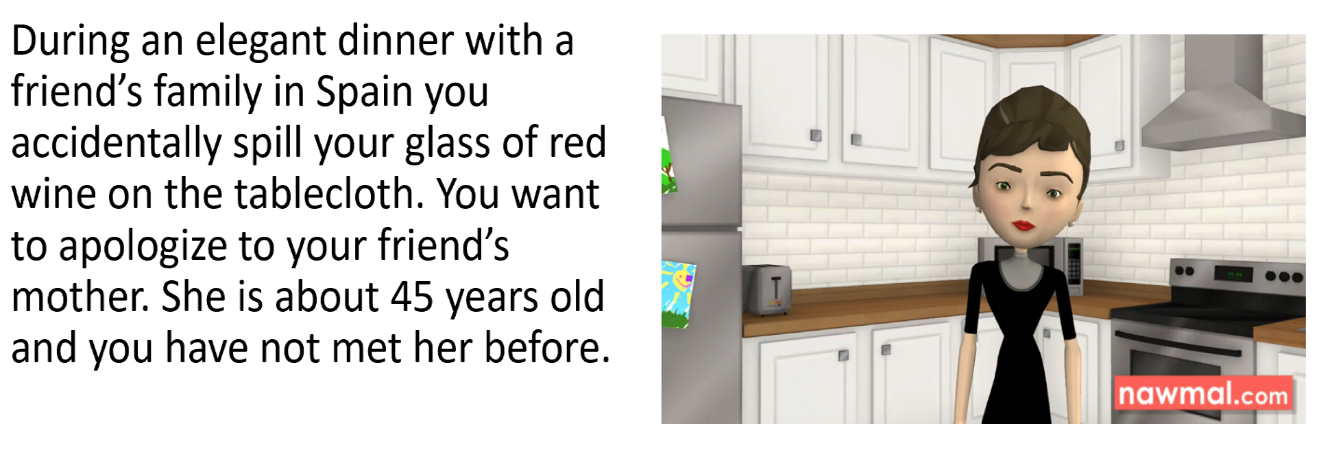
\includegraphics[width=\textwidth]{figures/rivera-img006.png}
\end{figure}


Naturalistic audio recordings, the fourth assessment method, have also been employed to measure L2 pragmatic development in the SA context (\citealt{BatallerShively2011,Dings2014,Dufon1999,Shively2011,Shively2013,Shively2015}). \citegen{Shively2011} SA participants made audio recordings of themselves while participating in service encounter interactions with service providers in Spain. In advocating for the use of naturalistic data for L2 pragmatics research, the author suggested that the service encounters analyzed had real-life interactional and psychological consequences. Similarly, according to \citet{BatallerShively2011}, naturally occurring data better capture how SA students interact in real-life encounters than do role-plays or production questionnaires. Although naturalistic data might represent a more valid measure of SA students’ pragmatic competence than other methods, several practice challenges exist in their application (e.g., comparability and unpredictability of data; time-consuming nature of data collection).

RVRs, the fifth assessment method, consist of obtaining verbal reports from a learner after completion of a task while information is still available in the learner’s short-term memory \citep{Félix-Brasdefer2010}. This procedure provides insights into the cognitive processes that learners employ while performing a task, such as information on their planning of a speech act, their language of thought, and their choice of language forms (\citealt{Ren2014,Woodfield2012}). RVRs are considered by some as essential for determining speech act performance because “one may learn what the respondents actually perceived about each situation (e.g., what they perceived about the relative role status of the interlocutors) and how their perceptions influenced their responses” (\citealt[321]{Cohen2004}). \citet{Woodfield2012} employed RVRs to investigate the perceptions of SA students with regard to their performance of two role-plays eliciting status-equal and status-unequal requests. The RVRs indicated that the students paid attention to linguistic form, sociopragmatic and pragmalinguistic knowledge, and politeness. The RVRs also suggested that it was often difficult for students to select appropriate forms to meet the goal of their interactions. Based on these findings, Woodfield concluded that RVRs help reveal learners’ current sociopragmatic and pragmalinguistic knowledge while informing researchers of the linguistic difficulties that learners face during speech act production.

Shifting to the sixth assessment method, some researchers have also employed native speaker perceptions of appropriateness as a measure of L2 learners’ pragmatic competence (e.g., \citealt{Halenko2018,Hernández2016,Hernández2018a,Hernándezinpress,HernándezBoero2018a,Li2014,ShivelyCohen2008,Taguchi2011}). \citet{Taguchi2006} defined pragmatic appropriateness as “the knowledge of the conventions of communication in a society, as well as linguistic abilities that enable learners to communicate successfully” (\citeyear[513]{Taguchi2006}). Criteria often used to assess appropriateness have included aspects of language use, level of formality, directness, politeness, word choice, and grammar \citep{Taguchi2011}. \tabref{tab:4:2} shows the appropriateness rating scale for requests designed by \citet{ShivelyCohen2008} and subsequently used by \citet{Hernández2016,Hernández2018a} and \citet{HernándezBoero2018a}. The reader interested in the speech act of apologies is directed to \citet{ShivelyCohen2008} for that rating scale.

\begin{table}
\fittable{
	\begin{tabular}{ll}
		\lsptoprule
		Rating & Descriptor \\
		\midrule
		5 & I would happily comply with the speaker’s request. \\
		4 & I would comply with the speaker’s request, but somewhat reluctantly. \\
		3 & I would comply with the speaker’s request, but reluctantly. \\
		2 & I would comply with the speaker’s request, but only very reluctantly. \\
		1 & I would not want to comply with the speaker’s request. \\
		\lspbottomrule
	\end{tabular}
	}
	\caption{\citegen{ShivelyCohen2008} pragmatic appropriateness rating scale for requests}
	\label{tab:4:2}
\end{table}

SA participants’ journal entries, the seventh assessment method, have been used in several studies to investigate L2 learners’ developing awareness of pragmatic norms (e.g., \citealt{Dufon1999,Hernández2018b,Shively2011}). As the eighth and final assessment method described in this chapter, audio recordings of tasks performed during the SA program have the potential to provide formative feedback to SA students and thereupon enhance their language acquisition. In \citet{HernándezBoero2018a}, participants were given tasks designed to strategically develop their pragmatic competence. Task performance was assessed by the researchers and explicit feedback was given to the L2 learners “to draw their attention to mismatches between their language use and pragmatic choices and those of the host culture” (\citeyear[396]{Hernández2018a}). DCTs have been one of the most frequently used methods to assess L2 pragmatic development in SA contexts for their ease of administration and ability to manipulate contextual variables (\citealt{Félix-BrasdeferHasler-Barker2017,RockeyEtAl2020}). To address some of the disadvantages of this instrument, researchers have begun to adopt other methods for evaluating pragmatic competence, such as role-plays, ODCTs, and naturalistic data, among others. Each also has its advantages and disadvantages. This chapter now shifts to a discussion of uninstructed and instructed L2 pragmatic development in SA.

\section{Uninstructed L2 pragmatic development in SA}

  Although studies on the development of pragmatic competence in the SA context have tended to focus on the investigation of speech acts (\citealt{KasperDahl1991,Ren2018}), other areas have also been researched: address forms (e.g., \citealt{Dufon1999,Hassall2013,Hassall2015b,Hassall2015a}); conversational style (e.g., \citealt{Cordelia1996}); humor \citep{Shively2013}; interactional competence (e.g., \citealt{Dings2014,Masuda2011,Shively2015,Shively2016,Taguchi2014development}); impoliteness \citep{Félix-BrasdeferHasler-Barker2017}; conversational implicature (e.g., \citealt{Taguchi2008a, Taguchi2008b}); and pragmatic routines (e.g., \citealt{AlcónSolerSánchezHernández2017,Osuka2014}). \tabref{tab:4:3} lists all existing research concerning uninstructed L2 pragmatic development during SA, published 1996 to 2021. Studies are organized by eight pragmatic features. Of these, the eighth, speech acts, is further subdivided into ten individual speech acts. For each study, the table presents author information (in alphabetical order), the target language, assessment methods employed by the researcher(s), and the duration of the SA program.

%\newcolumntype{L}{>{\raggedright\arraybackslash}p{3cm}}
%\setlength\LTleft{0pt}
%\setlength\LTright{-12pt}
%	{\small
%  \begin{xltabular}{.9\textwidth}{>{\raggedright\arraybackslash}p{2.5cm}lQp{2cm}}
%\begin{longtable}{>{\raggedright\arraybackslash}p{2.5cm}l>{\raggedright\arraybackslash}p{3.5cm}p{2cm}}
\begin{table}
\small
\begin{tabularx}{\textwidth}{>{\raggedright\arraybackslash}p{2.5cm}lQp{2cm}}
%		\caption{Studies on uninstructed pragmatic development in SA\label{tab:4:3}} \\
		\lsptoprule
%		Authors & Lang. & Assessment method & SA prog. dur.\\
%		\midrule\endfirsthead
%    \midrule
%    Authors & Lang. & Assessment method & SA prog. dur.\\
%		\midrule\endhead\endfoot
%    \lspbottomrule\\
%    \multicolumn{4}{>{\raggedright}p{\textwidth}}{\textsuperscript{\textit{a}} While \citet{Schauer2006,Schauer2009} focused on perception of appropriateness of requests in English, apologies, refusals, and suggestions were also investigated.}
%    \endlastfoot
  Authors & Lang. & Assessment method & SA prog. dur.\\
  \midrule
		\multicolumn{4}{l}{Pragmatic Feature 1: \textit{Address forms}} \\
%		\midrule
		\citet{Dufon1999}     & Ind & Naturalistic audio, recordings, DCT, journals                         & Semester  \\
		\citet{Barron2006}    & Ger     & DCT              							  & 1 year  \\
		\citet{Hassall2013}   & Ind & DCT, journals, interviews                    & 6 weeks \\
		\citet{Hassall2015b}  & Ind & DCT, journals, interviews      			  &	6 weeks \\
		\citet{Hassall2015a}  & Ind & DCT, journals, interviews      			  &	6 weeks \\
		\citet{Kinginger2008} & Fre     & Language awareness  interviews, journals, observations, role-plays      			  	  &	Semester  \\
		\midrule
		\multicolumn{4}{l}{Pragmatic Feature 2: \textit{Conventional expressions}} \\
%		\midrule
		\citet{Bardovi-HarligBastos2011} & Eng & Recognition and production tasks, language contact questionnaire    		  & Different  lengths  \\
	    \midrule
      \multicolumn{4}{l}{Pragmatic Feature 3: \textit{Conversational implicature}} \\
%	    \midrule
	    \citet{Taguchi2008a}  & Eng & Pragmatic comprehension and lexical tests, language contact questionnaire   & 4 months \\
	    \citet{Taguchi2008b}  & Eng & Listening task, language contact questionnaire    & 5--7 weeks   \\
		\midrule
\end{tabularx}
\caption{Studies on uninstructed pragmatic development in SA\label{tab:4:3}}
\end{table}
\begin{table}
\small
\begin{tabularx}{\textwidth}{>{\raggedright\arraybackslash}p{2.5cm}lQp{2cm}}
    \midrule
    Authors & Lang. & Assessment method & SA prog. dur.\\
    \midrule
		\multicolumn{4}{l}{Pragmatic Feature 4: \textit{Conversational style}} \\
%		\midrule
		\citet{Cordelia1996} & Spa  & ODCT 					      & Semester \\
		\citet{Iwasaki2008}  & Jpn & Oral proficiency interviews & 1 year \\
		\midrule
		\multicolumn{4}{l}{Pragmatic Feature 5: \textit{Humor}} \\
%		\midrule
		\citet{BellSalsbury2014}  & Eng & Informal conversations        & 10--12 months \\
		\citet{Kinginger2015} & Chi & Field notes, interviews,      & Summer      \\
							  &         & audio recordings			    &             \\
		\citet{Shively2013}   & Spa & Naturalistic audio recordings & Semester 	  \\
		\midrule
		\multicolumn{4}{l}{Pragmatic Feature 6: \textit{Impoliteness}} \\
%		\midrule
		\citet{Félix-BrasdeferMcKinnon2017} & Spanish & Impoliteness events & Semester \\
		\midrule
		\multicolumn{4}{l}{Pragmatic Feature 7: \textit{Interactional competence}} \\
%		\midrule
		\citet{Dings2014}    & Spa  & Audio recordings   & 1 year \\
		\citet{Ishida2010}   & Jpn & Naturalistic audio recordings & 1 year \\
		\citet{Masuda2011}   & Jpn & Audio recordings   & 6 weeks \\
		\citet{Shively2015,Shively2016} & Spa  & Naturalistic audio recordings & Semester \\
		\citet{Taguchi2014development}  & Jpn & Audio recorded conversations    & 12 weeks \\
		\midrule
		\multicolumn{4}{l}{Pragmatic Feature 8: \textit{Speech acts}} \\
%		\midrule
    \tablevspace
		\multicolumn{4}{l}{\textit{Apologies}} \\
%		\midrule
		\citet{Barron2019}       & Ger  & Corpus linguistics    & 10 months \\
		\citet{DiBartolomeoJung2019}         & Spanish & ODCT 			  	   & \\
		\citet{Hernández2018a}   & Spa & DCT            	   & 4 weeks \\
		\citet{Kondo1997}  	     & Eng & DCT				   & 1 year \\
		\citet{Schauer2006,Schauer2009}\textsuperscript{\textit{a}} & Eng & Video and questionnaire task & 9 months \\
    \citet{ShivelyCohen2008}     	 & Spa & DCT, language contact questionnaire & Semester \\
		\citet{WargaScholmberger2007} & Fre  & DCT            	   & 10 months \\
    \end{tabularx}
    \end{table}
    \begin{table}
    \small
    \begin{tabularx}{\textwidth}{>{\raggedright\arraybackslash}p{2.5cm}lQp{2cm}}
        \midrule
        Authors & Lang. & Assessment method & SA prog. dur.\\
        \midrule
%		\midrule
		\multicolumn{4}{l}{\textit{Compliments}} \\
%		\midrule
		\citet{Félix-BrasdeferHasler-Barker2015} & Spa & ODCT & 8 weeks \\
		\citet{Fukasawa2012} 	  & Eng & ODCT & 5 months \\
		\citet{Hoffman-Hicks1999} 		  & Fre  & DCT  & 16 months   \\
    \tablevspace
%		\midrule
		\multicolumn{4}{l}{\textit{Conventional and nonconventional speech acts}} \\
%		\midrule
		\citet{TaguchiLi2016} & Chi & ODCT & 3 months \\
    \tablevspace
%		\midrule
		\multicolumn{4}{l}{\textit{Giving advice}} \\
%		\midrule
		\citet{Matsumura2001,Matsumura2003} & & Judgment task & 1 year \\
    \tablevspace
%		\midrule
		\multicolumn{4}{l}{\textit{Gratitude}} \\
%		\midrule
		\citet{Cheng2005}  & 		 & DCT 			 & Different lengths \\
		\citet{DePablosOrtega2008} & Spa & Questionnaire & 3 months \\
    \tablevspace
%		\midrule
		\multicolumn{4}{l}{\textit{Greetings and leave-takings}} \\
%		\midrule
		\citet{Hoffman-Hicks1999}     & Fre  & DCT 					   & 16 months \\
		\citet{Kinginger2008} & Fre  & Language awareness, interviews, journals, observations, role-plays	   & Semester \\
    \tablevspace
%		\midrule
		\multicolumn{4}{l}{\textit{Offers}} \\
%		\midrule
		\citet{Barron2003,Barron2007} & Ger & DCT, RVRs, questionnaire    & 1 year \\
    \tablevspace
%		\midrule
		\multicolumn{4}{l}{\textit{Opinions}} \\
%		\midrule
		\citet{Taguchi2011} & Eng & ODCT & Cross-sectional \\
    \tablevspace
%		\midrule
		\multicolumn{4}{l}{\textit{Refusals}} \\
%		\midrule
		\citet{Barron2003,Barron2007}    & Ger  & DCT, RVRs, questionnaire         & 1 year \\
    \end{tabularx}
    \end{table}
    \begin{table}
    \small
    \begin{tabularx}{\textwidth}{>{\raggedright\arraybackslash}p{2.5cm}lQp{2cm}}
        \midrule
        Authors & Lang. & Assessment method & SA prog. dur.\\
        \midrule
		\citet{Félix-Brasdefer2004} & Spa & Role-plays, RVRs   & 1--30 months \\
		\citet{Félix-Brasdefer2013} & Spa & Role-plays, RVRs   & 8 weeks \\
		\citet{Ren2013} 	   & Eng & ODCT               & 1 year \\
		\citet{Ren2014}        & Eng & ODCT               & 10 months \\
		\citet{Schauer2006,Schauer2009}   & Eng & Video and questionnaire task     	  & 9 months\\
    \tablevspace
%		\midrule
		\multicolumn{4}{l}{\textit{Requests}} \\
%		\midrule
		\citet{Barron2003,Barron2006}  & Ger  & DCT            		& 1 year \\
		\citet{Bataller2010}  & Spa & Role-plays            & Semester \\
		\citet{Shively2011}   & Spa & Role-plays, naturalistic data          & Semester \\
		\citet{ColeAnderson2001}  & Eng & DCT                  	& 10 months \\
		\citet{CzerwionkaCuza2017a}     & 		& ODCT, judgment task   & 6 weeks \\
		\citet{CzerwionkaCuza2017b}     & 		& ODCT                  & 6 weeks \\
		\citet{Han2005}       & Eng & ODCT                  & 5 months to 5 years \\
		\citet{Hernández2016} & Spa & DCT, language contact questionnaire & 4 weeks \\
		\citet{Li2014}        & Chi & ODCT                  & Semester \\
		\citet{MagnanBack2006}      & Fre  & Role-plays            & Semester \\
		\citet{Ren2019}       & Chi & Role-plays            & Cross-sectional \\
		\citet{Rodríguez2001} & Spa & Judgment task, RVRs   & Semester \\
		\citet{Schauer2004}   & Eng & MET/ODCT              & 1 year \\
		\citet{Schauer2006,Schauer2009}  & Eng & Video and questionnaire task            & 9 months \\
		\citet{Schauer2007}   & Eng & MET/ODCT              & 9 months \\
		\citet{ShivelyCohen2008}     & Spa & DCT, language contact questionnaire & Semester \\
		\citet{Taguchi2011}   & Eng & ODCT          		& Cross-sectional \\
		\citet{VilarBeltrán2014}   & Eng & DCT, questionnaire    & Differentn lengths\\
		\citet{Woodfield2012} & Eng & Role-plays, RVRs & Semester \\
%    \tablevspace
%		\midrule
\end{tabularx}
\end{table}
\begin{table}
\small
\begin{tabularx}{\textwidth}{>{\raggedright\arraybackslash}p{2.5cm}lQp{2cm}}
    \midrule
    Authors & Lang. & Assessment method & SA prog. dur.\\
    \midrule
		\multicolumn{4}{l}{\textit{Suggestions}} \\
%		\midrule
		\citet{Schauer2006,Schauer2009} & Eng & Video and questionnaire tasks			 & 9 months \\
		\midrule
		\multicolumn{4}{l}{Pragmatic Feature 9: \textit{Pragmatic routines}} \\
%		\midrule
		\citet{AlcónSolerSánchezHernández2017} &	Eng		 & DCT             & Semester \\
		\citet{Osuka2014}     & Eng  & ODCT            & Semester \\
		\citet{Roever2012}    & Eng  & Web-based multiple choice       & Different lengths \\
		\citet{Taguchi2014production}   & Jpn & ODCT            & Different lengths \\
    \lspbottomrule
    \multicolumn{4}{>{\raggedright}p{\textwidth}}{\textsuperscript{\textit{a}} While \citet{Schauer2006,Schauer2009} focused on perception of appropriateness of requests in English, apologies, refusals, and suggestions were also investigated.}\\
\end{tabularx}
\end{table}
%	\end{xltabular}
%\end{longtable}
%}

\section{Development of receptive pragmatic competence in SA}

  This section provides an overview of studies that have investigated L2 learners’ development of receptive pragmatic competence in SA programs. SA participants made gains in their comprehension of leave-taking expressions (e.g., \textit{Au revoir.} ‘Goodbye’) and address forms in French \citep{Kinginger2008}, recognition of routine pragmatic formulae in English (\citealt{AlcónSolerSánchezHernández2017,Roever2012}) and Japanese \citep{Osuka2014}, and perception of speech acts in English (\citealt{VilarBeltrán2014,Schauer2006,Schauer2009}). In addition, increased pragmatic awareness regarding Spanish requests has also been observed (\citealt{CzerwionkaCuza2017a,Rodríguez2001}). \citegen{Rodríguez2001} investigation is particularly interesting because the author compared SA students with “at-home” learners over the course of a semester. Although data collected from a judgment task and RVRs demonstrated that both groups of learners improved their receptive ability of requests, no significant differences were found between the two groups. In another study on the acquisition of receptive skills, \citet{Taguchi2008a,Taguchi2008b} found that ESL learners’ gains in speed of comprehension of conversational implicatures over five months abroad were associated with self-reported language contact. Similarly, in \citegen{Matsumura2001} study, the improvements ESL learners made in their choice of appropriate advice-giving expressions were attributed to the amount of self-reported exposure to English. Meanwhile, \citet{Bardovi-HarligBastos2011} found that self-reported language contact had a positive effect on learners’ recognition and production of conventional expressions in L2 English. Length of residence, on the other hand, had no effect. The authors concluded that the quality of social contact while abroad was more important than length of residence when it comes to the development of conventional expressions.

\section{Development of productive pragmatic competence in SA}

\begin{sloppypar}
  As shown in \tabref{tab:4:4}, requests are the most investigated speech act in research on uninstructed L2 pragmatic development during SA (e.g., \citealt{Bataller2010,Han2005,Hernández2016,ShivelyCohen2008}). Researchers have examined other speech acts as well (e.g., \citealt{Félix-Brasdefer2004,Félix-Brasdefer2013,Hernández2018a,Hoffman-Hicks1999,Schauer2006}, \citealt{Schauer2009}). Employing the Cross-Cultural Speech Act Realization Project Coding Manual \citep{Blum-KulkaKasper1989} and \citegen{BrownLevinson1987} politeness theory as frameworks, several researchers have looked at how SA participants use (in)direct strategies, internal and external mitigation, formulas, semantic strategies, and deictic orientation in their speech acts before and after the SA program.
\end{sloppypar}

  Regarding apologies, some researchers have reported gains during SA \citep{WargaScholmberger2007}, whereas others have found little development of this particular speech act (e.g., \citealt{Hernández2018a,Kondo1997,ShivelyCohen2008}). One finding is conclusive: consistent with what has been observed for other areas of L2 learners’ pragmatic competence, the development of SA participants’ apologies is subject to significant individual variation. Using a DCT, \citet{Kondo1997} measured the development of L2 English apologies by Japanese high school learners before and after their academic year in the United States. The findings indicated that the participants became more target-like post-SA by shifting from overuse of Expressions of Apology (e.g., `sorry') to greater use of Explanations (e.g., I was late because there was an accident). Other forms of mitigation were also increased. \citet{Hernández2018a} found that 18 SA students did not improve several features of their Spanish apologies after short-term (4 weeks) SA. Students overused the expression of apology or illocutionary force indicating device (IFID), \textit{lo siento} (`I’m sorry'), on pre- and posttest DCTs. In contrast, they employed IFID Intensification (e.g., Lo \textit{siento de verdad.} `I’m truly sorry’) and the agentless construction in the Acknowledgement of Responsibility strategy (e.g\textit{., Se me olvidó~\ldots} `I forgot’) less frequently than the native speakers. Hernández concluded that exposure to target language input during SA may well be insufficient for participants “who have the expectation of acquiring the pragmatic features of the host community” (\citeyear[616]{Hernández2018a}). As such, the author argued that SA programs should incorporate explicit information about pragmatics into pre-departure orientation and again over the course of the experience abroad. Given the results of this study and others, pragmatic instruction might be particularly beneficial to SA participants in short-term programs.

  SA research indicates that L2 pragmatic development does not always occur in a linear fashion, as \citegen{WargaScholmberger2007} study of seven Austrian learners of French who studied for ten months in Quebec demonstrated. Three major developmental patterns were observed. First, SA participants became more target-like by reducing their use of Excuses and Justifications. Contrastively, the second development consisted of several shifts in the opposite direction of the target norm (e.g., increase in the use of two upgraders in one IFID). Third, during their program abroad the SA learners did not change their frequency of use of IFIDs, which they employed more frequently than the native speakers. An additional finding was the participants’ overuse of \textit{malheureusement} (‘unfortunately’) before SA. The authors suggested that they had transferred this strategy from their L1. During the second and third data collection times, the students decreased their use of \textit{malheureusement} and replaced it with target language chunks. By the fourth time, learners had begun to replace these target-like chunks with a more controlled and creative pragmatic performance. At this stage, the SA participants had combined native-like strategies with elements from their L1. The authors concluded that at the final stage of acquisition, the L2 learners would have target-like control of this feature. Employing corpus-based methods, \citet{Barron2019} investigated the development of L2 apologies by SA participants who spent ten months in Germany. The overuse of explicit IFIDs and single routine chunks were two of the pragmatic features that remained non-target-like over time.

  Turning to L2 request development, studies have found that SA participants improve in some aspects of their request behavior, as other features remain the same (e.g., \citealt{Barron2003}, \citealt{Barron2006,Bataller2010,ColeAnderson2001,Han2005,ShivelyCohen2008}). In their investigation of the requests and apologies of 67 American SA participants over the course of a semester, \citet{ShivelyCohen2008} found that although students improved their pragmatic appropriateness in some speech act scenarios, their formulation of requests and apologies was often non-target-like and at times even inappropriate. Two factors had a significant impact on specific speech act improvement:
  (1) the amount of time an SA participant spent speaking the target language outside of class with a fluent speaker of the L2, and
  (2) having extended conversations with the host family. \citet{Bataller2010} examined 31 US students’ requests in service encounters in a semester program in Spain. Results showed that SA participants overused non-target-like forms on the pre- and posttests, such as query permission (e.g., \textit{¿puedo tener una Coca-Cola?} ‘can I have a Coke?’), need statements (e.g., \textit{necesito} ‘I need’), unmitigated direct requests (e.g. \textit{quiero comprar otros zapatos} ‘I want to buy other shoes’). In addition, they did not increase their use of simple interrogatives (e.g., \textit{¿me pones un café?} ‘will you give me a coffee?’) or mitigated indirect request forms (e.g., \textit{quería cambiar estos zapatos} ‘I wanted to exchange these shoes’), which were the native Spanish speakers’ preferred strategies. Based on these findings, Bataller concluded that pragmatic instruction should be explicitly taught in SA programs so that students be made aware of the target pragmatic features and norms of the host culture.

  Using an ODCT, \citet{Li2014} examined how language proficiency influenced the development of pragmatic knowledge, as measured by appropriateness ratings, and processing ability, as measured by planning time and speech rate. In this study, American learners in both an Intermediate and Advanced group were rated as pragmatically more appropriate in their L2 Chinese request production after a semester sojourn abroad. Neither group reduced planning time. The Advanced group improved their speech rate, whereas the Intermediate group did not. Findings suggest that the broader pragmatic and linguistic knowledge base of the Advanced group helped them take advantage of the SA environment and thus continue to develop their processing ability and pragmatic knowledge. In a study on request development during short-term SA, \citet{Hernández2016} found that SA participants’ use of verbal downgrading (e.g., conditional or imperfect to express politeness or hedging) and external modification (e.g., explanations or justifications for a request) did not change from pre- to posttest. In addition, participants overused speaker-oriented forms (e.g., \textit{¿Puedo tener \ldots?} ‘Can I have?’) both before and after SA -- a phenomenon which researchers suggest is due to L1 transfer given that speaker-oriented requests are the norm in English (\citealt{Félix-Brasdefer2007,MárquezReiter2000,MárquezReiter2002,Pinto2005}). In his study, Hernández also measured the relationship between SA students’ amount of language contact and their request development. No significant relationships were found, however. The author concluded that traditional short-term SA experiences might not provide participants with adequate opportunities for practicing the target language in the host community. Similarly, \citegen{Taguchi2011} study on L2 English requests suggests that pragmatic gains made in SA may not be retained by L2 learners in the long-term.

  Refusals are another speech act that have received substantial attention in the SA literature (\citealt{Barron2003,Barron2007,Félix-Brasdefer2004,Félix-Brasdefer2013,Ren2014}). Employing role plays, \citet{Félix-Brasdefer2004} examined the relationship between SA participants’ development of Spanish refusals and their length of stay in the target language country. He found that learners with longer SA experiences (30 months abroad) had stronger control of mitigation in refusal sequences than those learners who had spent less time abroad. In a similar study, SA participants did not significantly improve their Spanish refusals after a much shorter program of eight weeks \citep{Félix-Brasdefer2013}. \citet{Ren2014} investigated the cognitive processes of advanced English language learners studying abroad for one academic year. Participants were given eight ODCT scenarios eliciting status-equal and status-unequal refusals in English. The results of the RVRs showed that, over time, learners paid increasingly more attention to sociopragmatics in context while increasing their pragmatic knowledge.

  Employing an ODCT, \citet{Félix-BrasdeferHasler-Barker2015} compared SA participants’ production of compliments in Spanish during an eight-week summer program in Mexico with students enrolled in an “at-home” context. Compliments involved four situations with differing degrees of social distance and power. The SA group showed some change with regard to one of the seven compliment strategies: \textit{Qué} ADJ/ADV NP (`What ADJ/ADV NP'). In addition, the SA participants more frequently employed \textit{padre} (‘cool’), an adjective type often used when making compliments in Mexican Spanish. In contrast, the AH group did not show significant change from pre- to posttest. Both groups overused \textit{Me} [\textit{gusta}, \textit{encanta}] NP (I [‘like, love’] NP). The authors attributed the L2 learners’ overreliance on this structure to three factors:
  (1) transfer (the English equivalent of this structure is frequent in English),
  (2) instruction (the dative Spanish structure is emphasized in the language curriculum), and
  (3) \citegen{Andersen1990} One-to-One Principle, which suggests that in the initial stages of language acquisition L2 learners tend to associate a structure with one function. Based on their findings, \citeauthor{Félix-BrasdeferHasler-Barker2015} concluded that “foreign language teaching as it stands is not sufficient to prepare learners to improve their pragmatic knowledge in specific areas, such as speech acts and other interactional routines. Although incidental learning in an SA setting helps improve the learner’s pragmatic competence, instruction in pragmatics before and during SA maximizes their learning experience. That is, without specific focus on both pragmalinguistic and sociopragmatic information and exposure to relevant pragmatic input, learners are not prepared to approach appropriate interactions with NS in the target language context” (\citeyear[85]{Félix-BrasdeferHasler-Barker2015}).

  Despite their importance for an L2 learners’ communicative competence, conversational style, address forms, and humor are three underrepresented areas in the SA literature (\citealt{Cordelia1996,Iwasaki2008,PérezVidalShively2019,Shively2011}). \citet{Cordelia1996} found that SA students who had spent time abroad acquired a confrontational style of speaking (e.g., cooperative overlap, challenging questions, and interruptions) similar to that of the native Spanish speakers. \citet{Hassall2013,Hassall2015a,Hassall2015b} examined the development of Indonesian address terms by Australian SA participants during a summer program abroad. Although the learners acquired new address terms for the vocative slot, their knowledge of terms for the pronoun slot increased only modestly. The author concluded that the SA students would have benefitted from pre-departure pragmatic instruction about address terms with opportunities to notice, reflect on, and discuss the L2 norms for their usage. With regard to L2 humor, \citet{Shively2013} followed an SA learner who developed his ability to be funny through participation in social interaction and feedback with age peers during one semester in Spain. Other studies (\citealt{BellSalsbury2014,Kinginger2015}) have also found a positive effect for SA on L2 humor development.

  Several studies have documented how L2 learners develop their interactional competence during SA (e.g., \citealt{Dings2014,Ishida2010,Masuda2011,Shively2015}, \citealt{Shively2016,Taguchi2014development}). \citet{Taguchi2014development} investigated the development of interactional competence by L2 learners of Japanese during their semester abroad in Japan. She found that over time her 18 SA participants increased their use of incomplete sentences, an important interactional resource in Japanese conversations because of its function in the joint construction of talk. \citet{Shively2015} examined listener responses (LRs) in Spanish during SA. She defined LRs as brief verbal responses (e.g., \textit{claro} ‘right,’ ‘of course’, \textit{ya} ‘right’) employed by a listener to provide feedback or support to the speaker, but which do not represent an attempt to take the floor or control topic development. LRs perform a wide range of functions essential for shaping ongoing discourse and developing intersubjectivity with the speaker: acknowledgement, understanding, receipt of previous talk, agreement, and evaluation. An analysis of 8,310 LRs revealed that over time the SA students shifted their use of speaker and listener responses in conversations with their native Spanish speaker interlocutors. However, because the SA group did not adopt allo-repetitions (e.g., repetition of all or part of a previous utterance) as a LR -- an important interactional resource more frequent in Spanish than in English -- Shively suggested that learners’ attention should be drawn to this particular strategy and other LR tokens through pedagogical intervention.

\begin{sloppypar}
  \citet{TaguchiLi2016} examined the effects intercultural competence and amount of social contact had on the development of pragmatic knowledge by 109 American college learners of Chinese participating in a semester program in Beijing. An ODCT consisting of 24 scenarios, a social contact questionnaire, and the Cross-Cultural Adaptability Inventory \citep{KelleyMeyers1995} were administered to participants pre- and post-program. Several important findings emerged from their analysis: First, the SA learners improved their speech act scores from pre- to posttest. Second, cross-cultural adaptability and social contact had a significant impact on pragmatic development. These findings are noteworthy because they suggest that to some extent SA participants’ individual characteristics (e.g., in this case their intercultural competence) influence their access to opportunities for language practice and subsequent increases in pragmatic knowledge, thus, accounting for some of the variation observed in SA pragmatic outcomes research.
\end{sloppypar}

\section{Instructed L2 pragmatic development in SA}

\begin{sloppypar}
  Studies on uninstructed L2 pragmatic development in SA environments have demonstrated that some students make progress in acquiring the pragmatic norms of the host culture (e.g., \citealt{ShivelyCohen2008}). At the same time however, not all L2 learners improve their pragmatic competence (e.g., \citealt{Bataller2010,Hernández2018a,ShivelyCohen2008}). Even fewer acquire native-like pragmatic ability. Social contact is one of several factors that has been identified as contributing to SA participants’ pragmatic development. Length of stay represents another important factor that may affect acquisition. SA students in short-term programs are at a potential disadvantage because of the inadequate exposure to the target language. Exacerbating these disadvantages, researchers have observed that even highly motivated students are often unaware of how to take full advantage of the SA environment for developing their pragmatic competence (\citealt{CohenShively2007,HernándezBoero2018a,Shively2010}). As a result, in order to maximize outcomes, some researchers have advocated for the integration of classroom-based pragmatic instruction into SA programs because explicit instruction has been found to promote learners’ pragmatic development \citep{Martínez-FlorUsó-Juan2006}.
\end{sloppypar}

  Pragmatics instruction in SA contexts has tended to employ an awareness-raising approach to developing pragmatic competence (\citealt{HalenkoJones2017,HernándezBoero2018a,HernándezBoero2018b,HernándezBoero2019,Martínez-FlorUsó-Juan2006,Shively2010}). According to \citet{Schmidt2001}, there must be conscious noticing of a given target feature in the input for acquisition to occur. In the case of pragmatics, L2 learners must notice and understand not only linguistic form, but also pragmalinguistic function \citep{Morris2017}. Because previous studies have shown that left to their own devices SA participants often lack the strategies to take full advantage of the SA context for developing their pragmatic skills (\citealt{CohenShively2007,Hernández2016,Hernández2018a,PérezVidalShively2019,Shively2010,ShivelyCohen2008}), researchers have begun to investigate the effects of pre-departure and in-country pedagogical intervention on L2 learners’ pragmatic development. \tabref{tab:4:4} lists all extant research assessing the impact of pedagogical intervention on SA participants’ pragmatic competence, published between 1996 and 2020. Studies are organized by three pragmatic features. The third feature, speech acts, is thereupon subdivided into four individual speech acts. For each study, the table presents author information (in alphabetical order), the target language, assessment methods employed by the researcher(s), and the duration of the SA program.

\begin{table}
\small
	\begin{tabularx}{\textwidth}{p{4cm}lQl}
		\lsptoprule
		Authors & Language & Assessment method & \makecell[tl]{SA prog.\\duration} \\
		\midrule
		\multicolumn{4}{l}{Pragmatic Feature 1: \textit{Address forms}} \\
%		\midrule
		\citet{Henery2015} & French & Awareness  & Semester \\
						   &		& interviews & \\
		\midrule
		\multicolumn{4}{l}{Pragmatic Feature 2: \textit{Conversational implicatures}} \\
%		\midrule
		\citet{Bouton1999} & English & Questionnaire & 1 year \\
		\midrule
		\multicolumn{4}{l}{Pragmatic Feature 3: \textit{Speech acts}} \\
%		\midrule
    \tablevspace
		\multicolumn{4}{l}{\textit{Apologies}} \\
%		\midrule
		\citet{CohenShively2007} & \makecell[tl]{French/\\Spanish} & DCT, language contact questionnaire & Semester \\
		\citet{Halenko2018}  & English &  ODCT & Summer \\
		\citet{Hernándezinpress} & Spanish &  ODCT & 4 weeks \\
%		\midrule
    \tablevspace
		\multicolumn{4}{l}{\textit{Complaints}} \\
%		\midrule
		\citet{RussellVásquez2018} & Spanish & DCT & \makecell[tl]{Semester \\prior to SA} \\
%		\midrule
    \tablevspace
		\multicolumn{4}{l}{\textit{Compliments}} \\
%		\midrule
		\citet{DiBartolomeoJung2019} & Spanish & ODCT & 5 weeks \\
		\citet{Mir2020}    			 & Spanish & ODCT & 4 weeks \\
%		\midrule
    \tablevspace
		\multicolumn{4}{l}{\textit{Requests}} \\
%		\midrule
		\citet{CohenShively2007}              & Spanish & DCT   				   & Semester \\
		\citet{HalenkoJones2011}              & English & DCT           		   & 12 weeks \\
		\citet{HalenkoJones2017}              & English & ODCT            		   & 6 months \\
		\citet{Hernández2018b}                & Spanish & Role-plays, journals     		   & 6 weeks \\
		\citet{HernándezBoero2018a}           & Spanish & DCT, RVRs                & 4 weeks \\
		\citet{HernándezBoero2018b}           & Spanish & Role-plays               & 5 weeks \\
		\citet{HernándezBoero2019}            & Spanish & DCT                      & 4 weeks \\
		\citet{Morris2017}\footnote{\citegen{Morris2017} DCT focused on requests. Greetings, invitations, closings, and refusals were also measured.} & Spanish & DCT                      & 10 weeks \\
		\citet{RussellVásquez2018}            & Spanish & DCT, com\-pre\-hen\-sion-based assessment	   & \makecell[tl]{Semester\\prior to SA} \\
		\citet{Shively2011} 				  & Spanish & Naturalistic  		   & Semester \\
											  &			& recordings			   & \\
		\citet{WinkeTeng2010} 				  & Chinese & ODCT, journals           & 8 weeks \\
		\lspbottomrule
	\end{tabularx}
	\caption{Studies on instructed pragmatic development in SA}
	\label{tab:4:4}
\end{table}




\section{Instructed pragmatic development in SA: Development of receptive pragmatic competence}

  To date only two empirical studies that the author is aware of have investigated the effects of explicit pragmatic instruction on developing receptive skills of students in the SA context (\citealt{Bouton1999,Henery2015}). Consisting of six hours of instruction, \citegen{Bouton1999} pedagogical intervention was effective in helping SA participants acquire conversational implicatures in English. \citet{Henery2015} found that SA students who received guidance from an instructor developed their metapragmatic awareness of French (i.e., address forms and understanding of contextual factors that inform language choices) more than those participants who did not receive guidance. Her findings suggest that SA programs should encourage students to make linguistic observations during their time abroad while an expert instructor guides and scaffolds their interpretations.


\section{Instructed pragmatic development in SA: Development of productive pragmatic competence}

  Existing research assessing the impact of pragmatics instruction on SA students’ productive pragmatic skills suggests that pragmatics instruction is beneficial (e.g., \citealt{CohenShively2007,DiBartolomeoJung2019,Halenko2018,HernándezBoero2018a,HernándezBoero2018b,Morris2017,Shively2011}). Employing DCTs, \citet{CohenShively2007} examined the impact of pedagogical intervention on 86 US students’ acquisition of requests and apologies during a semester abroad in a French or Spanish-speaking country. In their pre-departure orientation, the experimental group received presentation, discussion, and practice activities on learning how to perform speech acts in the target language. Participants responded to practice scenarios, and then compared their answers to those of their peers. Next, the students compared their responses to native speakers of French or Spanish who had also completed the same speech act scenarios. While abroad, the experimental group wrote reflective e-mail journals about their language learning during the SA experience. The control group did not receive instruction on speech acts nor did they write journal entries. Although both groups increased their use of target-like speech act strategies, as measured by a production questionnaire, there was no significant effect for the intervention. Based on these findings, Cohen and Shively concluded that pragmatics instruction should consist of a more extensive intervention during pre-departure orientation. While abroad, SA participants should also be given practice activities that encourage noticing and reflection on pragmatic features.

  In a study employing naturalistic data, \citet{Shively2011} reported on the service encounter requests of seven SA students who spent a semester in Spain. A total of 131 audio recordings between the SA participants and service providers in Spain were analyzed. Results showed that the students shifted from speaker-oriented requests (e.g., \textit{¿puedo tener un café?} ‘Can I have a coffee?’) to greater use of hearer oriented (\textit{¿me pones un café?} ‘Will you give me a coffee?’) and elliptical forms (e.g., \textit{un café, por favor} ‘A coffee, please’). In their journal entries and in interviews with the researcher, the SA learners attributed their improvement to the explicit information about pragmatics they received during the first and fifth weeks of the semester and to socialization with the host community.

  \citet{HalenkoJones2017} assessed the impact of pre-departure instruction on SA participants’ production of requests by Chinese learners of English. Requests were measured by an ODCT administered as a pretest, posttest, and delayed posttest. Findings indicated that explicit instruction had a significant effect on the immediate posttests. Significant attrition was found on the delayed posttests, however. The authors concluded that regular, repeated metapragmatic instruction might have had a more positive impact on SA students’ acquisition of pragmatic features than the practice given to them within a short time period.

  In a similar study, \citet{Halenko2018} investigated the efficacy of an ODCT for assessing and improving the spoken communication skills of Chinese learners of ESL during their UK-based SA program. ESL learners were assigned to either an experimental group who received computer-assisted explicit instruction on apologies, or a control group that did not receive instruction. The instruction followed \citegen{Uso-Juan2010} five stages of awareness-raising and communicative practice. In stage one, learners were introduced to the linguistic and cultural aspects of the speech act of apologizing. During stage two, they were presented with the formulaic expressions used to offer apologies. In the third stage, the researcher provided the learners with authentic scenarios designed to encourage reflection on aspects associated with \citegen{BrownLevinson1987} politeness theory, such as power, distance, and imposition -- and their relationship to speech act production. ESL learners then engaged in communicative practice in stage four, followed by teacher-led discussion and feedback in stage five. ODCT data showed that computer-assisted explicit instruction and practice was indeed an effective tool for developing and assessing the SA participants’ pragmatic development of L2 apologies.

\begin{sloppypar}
  \citet{Morris2017} examined the effects of a task-based intervention on the pragmatic development of twelve SA participants during a ten-week program in Spain. Pragmatic development was measured by pre- and posttest DCTs, audio recordings of tasks performed in the target culture community, and self-reflections of task performance. Participants demonstrated significant gains in pragmatic competence (e.g., giving directions and ordering meals in Spanish) on the DCT and in their task completion. Similarly, their reflections showed increased awareness of the pragmatic features introduced to them during the entire pedagogical intervention. Using an ODCT and journaling, \citet{WinkeTeng2010} measured the impact of task-based pragmatics instruction during an SA program in China. SA participants improved their use of formulaic expressions in speech act production. In addition, students’ journal entries revealed developing awareness of Chinese pragmatics.
\end{sloppypar}

  \citet{HernándezBoero2018a} found a positive effect for pragmatics instruction in the short-term SA context. Prior to departure, 15 SA participants received explicit instruction on requests, then guided practice with authentic input and awareness-raising activities, output practice, and subsequent group discussion and feedback. In Spain, they performed four simulated tasks that required them to make requests. The tasks varied in terms of social distance, social status, and degree of imposition. Next, the SA participants responded to questions that encouraged reflection about the appropriateness of their request strategies. Feedback was also given. In addition to significant gains on posttest DCTs, RVRs demonstrated that specific sociopragmatic factors and pragmalinguistic strategies targeted during the intervention informed learners’ cognition during speech act planning and production.

  In another investigation on short-term SA, \citet{HernándezBoero2019} employed DCTs to measure participants’ request making in two service encounter scenarios. The first scenario was ordering a drink at a café. The second involved exchanging a pair of shoes without having the receipt. The SA participants made significant gains in both scenarios. \citet{HernándezBoero2018b} found that the positive effects of their pragmatic intervention extended to students’ request production in role-plays. In addition, most of the gains were retained in delayed posttests administered five weeks after the conclusion of the SA program. The authors attributed the SA participants’ gains in the long term to the repeated exposure to pragmatics instruction that the L2 learners received during their entire time abroad. Employing role-plays, \citet{Hernández2018b} examined the effects of pedagogical intervention on SA participants’ requests during a six-week program in Buenos Aires, Argentina. Findings again demonstrated that explicit pragmatic instruction combined with in-country pragmatic data gathering tasks contributed to the students’ L2 pragmatic development.

  \citet{RussellVásquez2018} examined the impact of a web-based tutorial (WBT) on 13 US students’ pragmatic development during the semester prior to studying abroad in Spain. Findings indicated that the SA participants slightly increased their use of pragmatically appropriate strategies on the posttest production questionnaire, especially in the area of conventional politeness formulae to frame a complaint. Pre- and posttest scores on a comprehension-based assessment revealed that their ability to comprehend or notice appropriate pragmatic strategy use in Spanish also improved. The authors concluded that instruction on specific grammatical features taught in context prior to the WBT -- such as the past subjunctive and conditional mood in Spanish -- may help students formulate more appropriate hedges and downgraders in their speech act production. \citet{DiBartolomeoJung2019} reported on SA students’ compliments and apologies after five weeks in Mexico. Over the course of their time abroad, participants received pragmatic instruction on compliments but not on apologies. Most of the SA learners improved their use of compliments. In contrast, few students adopted the native norms for apologies in Spanish. The authors concluded that the pragmatic instruction was responsible for the differential outcomes observed at the time of the posttests.

\citet{Hernándezinpress} considered multiple measures of pragmatic knowledge in his investigation on the effects of pedagogical intervention and short-term SA on the development of L2 Spanish apologies. Students who spent four weeks in different SA programs in Spain were randomly assigned to an experimental group (\textit{n}~=~9) or a control group (\textit{n}~=~9). Prior to departure, the experimental group received explicit pragmatic instruction on how to formulate apologies. During SA, they performed two task scenarios designed to improve their pragmatic competence. The control group did not receive explicit pragmatic instruction, nor did they perform the tasks. L2 pragmatic development was assessed by an ODCT consisting of five apology scenarios. The ODCT data demonstrate that the experimental group significantly outperformed the control group in three measures of pragmatic development: appropriateness ratings by native speakers, strategy use, and speech rate. The agentless construction in the Acknowledgement of Responsibility strategy (e.g., \textit{Se me cayó} `I dropped') and IFID Intensification (e.g., \textit{Lo siento de verdad.} ‘I’m truly sorry’), two problematic structures for L2 Spanish learners, were among the features that the experimental group increased on the posttests. The experimental group also reduced their use of the single chunk \textit{lo siento} `I’m sorry' while expanding their IFID repertoire (e.g., \textit{Perdóneme.} ‘Excuse me’). In contrast, the control group did not improve their apologies during SA, often overusing routine expressions.

\citet{Mir2020} examined the impact of pedagogical intervention on SA participants’ L2 Spanish compliments during a four-week program in Spain. Data were collected by an ODCT consisting of eight complimenting scenarios. Over the course of the first two weeks, 20 students received explicit instruction on Spanish pragmatics, with a focus on speech act of compliments and compliment responses. Next, they were asked to conduct ethnographic research in the host community. Activities included: (1) asking their host families to perform several role-plays, which the students recorded and thereupon transcribed; (2) recording, transcribing, and analyzing conversations in the host community; and (3) practice employing compliments and compliment responses with host family members. For all three tasks, the SA participants shared the information they gathered from the native informants in subsequent class discussions focusing on pragmatics. Weekly journal entries were also employed to provide learners with further opportunities to discuss and interpret the pragmatic data. The ODCT data show that the explicit classroom-based pragmatic instruction combined with the ethnographic work helped the SA participants develop target-like complimenting strategies (e.g., \textit{Que} + ADJ/NP construction) on the posttests.

\begin{sloppypar}
  Although studies on instructed L2 pragmatic development have predominantly focused on pragmatic speaking ability, \citet{Alcón-Soler2015} conducted a unique study on the assessment of writing skills in L2 English. Specifically, the author investigated the impact of pragmatics instruction on learners’ ability to mitigate requests in e-mail communication with their instructors. The experimental group received instruction on e-mail requests in which their attention was drawn to request forms, sociocultural norms, and discourse structure in academic e-mail communication. In addition, this group was provided with practice and feedback. The control group did not receive instruction but did exchange e-mails with their instructor. Although the quantitative analysis showed that both groups improved on the posttests, the qualitative analysis revealed that the experimental group had a more developed understanding of the relationship between forms and context.
\end{sloppypar}

  \citet{Shively2010} provided the most comprehensive model to date for teaching pragmatics prior to, during, and after SA. During pre-departure, SA participants learn the relevance of pragmatics for SA. The primary goal of this stage is to build the L2 learners’ confidence in the target language so that they can maximize their SA experience. Participants’ attention is drawn to the pragmatic norms (e.g., norms about interaction in the target language) of the host culture. Communicative practice with speech acts is another core component of Shively’s pre-departure stage. While abroad, SA students are encouraged to notice, reflect, and consider pragmatic features in out-of-class data gathering activities and with the guidance of an instructor or program director. The post-SA component of this model involves facilitating former SA students’ “social interaction in the target language and continued development of the skills acquired in both the pre-departure and in-country stages” (\citeyear[123]{Shively2010}).

\section{Conclusions and future directions}

  In this chapter, I have provided an overview of studies that have measured L2 pragmatic development in SA contexts. First, I discussed the major assessment methods that have been employed to measure pragmatic knowledge in the SA environment. I then reviewed the existing scholarship on SA participants’ acquisition of pragmatic competence in both uninstructed and instructed environments. The SA literature has demonstrated that some L2 learners improve some aspects of their pragmatic competence while participating in a sojourn abroad of a semester or more. Other pragmatic features develop slowly or are difficult to acquire through exposure alone. One important insight gained from assessment on SA students’ L2 pragmatic development is that pedagogical intervention before and during SA has the potential to enhance pragmatic learning. Furthermore, as participation in short-term SA increases \citep{InstituteofInternationalEducation2017}, more studies should assess the impact that these programs have on participants’ L2 pragmatic ability. Research suggests that students in these programs would benefit from instruction on pragmatic features during pre-departure orientation and subsequent opportunities to notice, practice, reflect on, and receive feedback about speech patterns during the SA program (e.g., \citealt{HernándezInPress,HernándezBoero2018a,HernándezBoero2018b}).

With respect to assessment methods, researchers have begun to shift away from written production questionnaires or DCTs, which are perceived as having lower validity compared to other measures of pragmatic competence (\citealt{Félix-Brasdefer2010,PérezVidalShively2019}). ODCTs and role-plays are two such measures that may be better suited for capturing L2 learners’ language use in social contexts. Although \citet{RockeyEtAl2020} did not focus on SA participants’ pragmatic competence, their study on technology-enhanced (TE) DCTs demonstrates how researchers might employ a mobile application to increase the validity of traditional DCTs in SA contexts as well. In their study, the use of a TE-DCT accessed by a phone application provided students not only with important linguistic and extralinguistic cues, but it also allowed them to employ these same features in their own responses. Based on this data, the authors argued that the use of mobile applications was an ecologically valid way to measure one type of pragmatic ability. In addition to issues surrounding increased face and content validity, TE-DCTs would also enhance researchers’ ability to collect L2 pragmatic data from SA participants in different programs. RVRs also offer a potentially rich source of data about how SA learners perceive social and cultural variables associated with different speech acts. Naturalistic data, for their part, allows programs to investigate how SA participants make use of their pragmatic skills in authentic situations. Asking SA participants to become data gatherers is one approach to obtaining authentic interactional data (e.g., \citealt{Shively2011}). A second approach is to analyze how students use the target language in social media and chat applications such as Facebook, Instagram, or WhatsApp \citep{PérezVidalShively2019}.

In terms of directions for future research, a worthwhile avenue of investigation would be to use a simulated 3-D SA environment (e.g., with actors from the target language country and simulated situations and surroundings) as pre-departure practice, and also as a method for measuring participants’ L2 pragmatic competence before and after an SA program. Given the increasing interest in SA programs with service learning, internships, volunteering, and work placement (e.g., an SA program designed for nurses; Engineers without Borders), research in this area is especially relevant. Similarly, researchers could combine this assessment method with measurements of stress or situational anxiety -- an approach that has been identified in recent discussions about pragmatics in the SA context \citep{PérezVidalShively2019}.

Most of the research on uninstructed L2 pragmatic development in SA has focused on speech acts (e.g., \citealt{Félix-BrasdeferHasler-Barker2015,Hernández2016,Hernández2018b,Ren2014,Ren2019,ShivelyCohen2008}). Although these studies have contributed important information about what SA students can and cannot acquire during their time abroad, other aspects of pragmatics should also be investigated. L2 learners’ interactional competence (e.g., discursive abilities, discourse marker use, backchanneling) and pragmatic processing ability (e.g., \citealt{Hernándezinpress,Li2014}) are two areas that merit further attention.

It should also be noted that the difficulties of measuring L2 pragmatic competence are exacerbated by the fact that some L2 learners may consciously use a non-target-like feature because they know it is correct even though it is not pragmatically appropriate. \citet{Barron2003} referred to this phenomenon as the “playing it safe” strategy. Finally, language contact and motivation are often identified as important predictors of language acquisition in the SA context. However, with the exception of a few studies (e.g., \citealt{Bardovi-HarligBastos2011,Hernández2016,Matsumura2001,ShivelyCohen2008,Taguchi2008a,Taguchi2008b}), research on how students’ self-reported language contact or social networks influence L2 pragmatic development is underrepresented. Research that measures how individual differences influence the path of L2 pragmatic development that an SA learner takes in acquiring pragmatic competence during SA represents another important line of investigation.

The positive effects of pragmatics instruction on SA participants’ developing pragmatic competence are promising. The focus of these studies has also been on speech acts, however. More research is needed on the impact of explicit classroom-based pragmatic instruction on other pragmatic features as well. Further, few studies have examined the impact of an intervention that takes place both before and during SA (e.g., \citealt{Hernándezinpress,HernándezBoero2018a,Shively2011}). Given that these interventions seem to be more beneficial for SA students’ pragmatic development than pre-departure-only instruction, additional studies are justified. At the same time, further research on pedagogical interventions that encompasses not only these two important SA stages (pre-departure and in-country), but also examines post-SA pragmatic development is also warranted. Finally, assessment of L2 pragmatic development in SA has demonstrated that the “at-home” foreign language curriculum does not adequately prepare L2 learners to improve “their pragmatic knowledge in specific areas, such as speech acts and other interactional routines” (\citealt[85]{Félix-BrasdeferHasler-Barker2015}). A language curriculum that targets the development of learners’ pragmatic competence well before SA and then continues to build on this knowledge in pre-departure and during the program itself will help SA participants maximize their learning experience. Systematic assessment of SA outcomes will undoubtedly assist with this effort.

\sloppy
\printbibliography[heading=subbibliography,notkeyword=this]

\end{document}
